% !TEX program = xelatex
% ============================================================================
% Overleaf 설정: Menu > Compiler > XeLaTeX (또는 LuaLaTeX)
% kotex이 한글을 처리하므로 pdfLaTeX로는 컴파일되지 않는다.
%
% 파일 구조(2026-08-17 다중 파일로 재구성 — 내용은 그대로, 파일만 분리):
%   preamble/packages.tex  — \usepackage 전부
%   preamble/layout.tex    — 여백/줄간격/제목 간격
%   preamble/commands.tex  — \todo, \chk 커스텀 명령
%   sections/00_front.tex      — \maketitle + abstract
%   sections/01_introduction.tex
%   sections/02_related_work.tex
%   sections/03_protocol.tex
%   sections/04_results.tex
%   sections/05_failure_analysis.tex
%   sections/06_guideline.tex
%   sections/07_conclusion.tex
%   sections/08_appendix.tex   — bibliography
% ============================================================================
\documentclass[11pt]{article}

% ---- 한글 및 기본 ----------------------------------------------------------
\usepackage{kotex}
\usepackage{amsmath, amssymb, mathtools}
\usepackage{graphicx}
\usepackage{xcolor}

% ---- 표 ---------------------------------------------------------------------
\usepackage{booktabs}
\usepackage{multirow}
\usepackage{array}
\usepackage{tabularx}
\newcolumntype{L}[1]{>{\raggedright\arraybackslash}p{#1}}

% ---- 캡션/리스트 -------------------------------------------------------------
\usepackage[font=small, labelfont=bf, skip=4pt]{caption}
\captionsetup[table]{position=top}
\captionsetup[figure]{position=bottom}

\usepackage{enumitem}
\setlist{itemsep=0.35em, topsep=0.5em, parsep=0pt}

\usepackage{microtype}               % 자간 미세 조정 (가독성)

% ---- 링크 -------------------------------------------------------------------
\usepackage[colorlinks=true, linkcolor=black, citecolor=black,
            urlcolor=blue!60!black]{hyperref}

% ---- 레이아웃 및 간격 -------------------------------------------------------
% 2026-08-19: 10--11장 분량 목표로 여백/줄간격/문단간격/float 주변 여백을 전반적으로
% 소폭(10~25%) 줄였다 — 어느 하나를 무리하게 줄이지 않고 여러 군데를 조금씩 줄이는
% 방식(자간 자체는 건드리지 않음, 폰트 크기·글자 사이 간격은 그대로).
\usepackage[margin=0.85in]{geometry}
\setlength{\columnsep}{0.26in}       % 2단 사이 간격(가운데 기준선)
\usepackage{setspace}
\setstretch{1.08}                    % 줄 간격(1.15 -> 1.08)
\setlength{\parskip}{0.42em}         % 문단 간격(0.55em -> 0.42em)
\setlength{\parindent}{1em}          % 들여쓰기

% float(그림/표) 주변 여백 축소 — 기본값(약 12--20pt)보다 타이트하게.
\setlength{\textfloatsep}{10pt plus 2pt minus 2pt}
\setlength{\dblfloatsep}{10pt plus 2pt minus 2pt}
\setlength{\intextsep}{8pt plus 2pt minus 2pt}
\setlength{\floatsep}{8pt plus 2pt minus 2pt}

\usepackage{titlesec}
\titlespacing*{\section}      {0pt}{1.5em}{0.7em}
\titlespacing*{\subsection}   {0pt}{1.1em}{0.45em}
\titlespacing*{\subsubsection}{0pt}{0.9em}{0.4em}
\titlespacing*{\paragraph}    {0pt}{0.8em}{0.6em}
\titleformat{\paragraph}[runin]{\normalfont\bfseries}{}{0pt}{}[.]

% ---- 절 번호 체계(2026-08-18, 학회 양식 대조) -------------------------------
% \section은 로마 숫자(중앙 정렬), \subsection은 그 절 안에서 다시 1부터 시작하는
% 아라비아 숫자(왼쪽 정렬, 제목 앞) — GSSS 학회 양식(예: "I. 서론", "III. 실험 프로토콜"
% 안의 "1. 공정성 원칙") 대조. \thesubsection 자체는 article.cls 기본값
% (\thesection.\arabic{subsection}, 예: "IV.5")을 그대로 둔다 — \S\ref{}로 본문에서
% 절을 가리킬 때는 "§IV.5"처럼 로마 숫자 절 번호까지 나와야 하기 때문이다(제목에 찍히는
% 번호만 아래 \titleformat에서 절 번호를 뺀 순수 \arabic{subsection}으로 바꾼다).
\renewcommand{\thesection}{\Roman{section}}
\titleformat{\section}{\centering\normalfont\large\bfseries}{\Roman{section}.}{0.6em}{}
\titleformat{\subsection}{\normalfont\bfseries}{\arabic{subsection}.}{0.5em}{}
\renewcommand{\refname}{References}

% ---- 사용자 명령 ------------------------------------------------------------
\newcommand{\todo}[1]{\textcolor{red}{\textbf{[TODO: #1]}}}
\newcommand{\chk}[1]{\textcolor{orange!80!black}{\textbf{[확인: #1]}}}


% ============================================================================
\title{Sparse-view 3D Gaussian Splatting에서\\
       Feed-forward와 장면별 최적화의 우위 조건 분석}
\author{\todo{저자명 / 소속}}
\date{\today\ \ (초안 — 실험 진행 중)}

\begin{document}

\maketitle

\begin{abstract}
사진 몇 장으로 3D 장면을 재구성하는 방법은 크게 두 갈래로 나뉜다. 하나는 미리 학습한 모델에 사진을 넣으면 즉시 3D Gaussian을 출력하는 feed-forward 방식이고, 다른 하나는 새 장면마다 그 장면 전용으로 반복 최적화하는 per-scene optimization 방식이다.

본 연구는 새로운 알고리즘을 제안하는 대신, \textbf{입력 view 수, view 간 겹침 정도(co-visibility overlap), 사용 가능한 계산 시간 예산}을 통제 축으로 삼아 대표 시스템들(feed-forward: MVSplat~\cite{chen2024mvsplat}, DepthSplat~\cite{xu2025depthsplat}; per-scene optimization: 3D Gaussian Splatting~\cite{kerbl20233d}, FSGS~\cite{zhu2024fsgs})의 실용적 우위 지도(regime map)를 그린다.

동일한 feed-forward 초기값에서 표준 3DGS refinement를 켜고 끄는 통제 실험으로 최적화의 순효과를 분리하고, 카메라 기하학 기반 불확실도 분석과 통제된 depth noise 개입으로 우위가 갈리는 원인을 설명하며, 마지막으로 조건별 선택 가이드라인을 제시한다. \todo{실험 완료 후 핵심 수치 1--2개를 요약에 추가}
\end{abstract}

\noindent\todo{본 문서는 실험이 진행 중인 상태의 초안이다. 표/수치가 비어 있는 절은 명시적으로 표시했다. 산문(서론, 관련 연구, 프로토콜, 일부 분석)은 지금까지 확정된 내용을 담았다.}

% =====================================================================
\section{서론}
\label{sec:intro}
% =====================================================================

Sparse-view(입력 사진이 매우 적은) 조건에서 3D 장면을 재구성하는 문제는 서로 다른 두 계열의 접근으로 발전해 왔다. 첫 번째는 3D Gaussian Splatting~\cite{kerbl20233d}으로 대표되는 \emph{per-scene optimization} 계열로, 각 장면마다 처음부터 반복적인 경사하강법으로 Gaussian 파라미터를 학습한다. 사진이 충분하고 시간이 허락되면 매우 높은 품질의 재구성을 얻을 수 있지만, sparse-view 조건에서는 초기화가 빈약하고 관측이 부족해 densification이 불안정해지는 것으로 알려져 있다.

두 번째는 pixelSplat~\cite{charatan2024pixelsplat}, MVSplat~\cite{chen2024mvsplat}, DepthSplat~\cite{xu2025depthsplat} 등으로 대표되는 \emph{feed-forward} 계열로, 사전 학습된 신경망이 입력 사진에서 단일 forward pass로 3D Gaussian을 직접 예측한다. 추론이 매우 빠르고 sparse-view에 강인하지만, 학습 시 본 입력 분포(view 수, 데이터셋)를 벗어나면 성능이 급격히 저하되는 한계가 있다.

두 계열의 경계 지대는 최근 활발한 연구 대상이다. 예를 들어 feed-forward 예측을 초기값으로 삼아 짧은 per-scene 정제를 수행하는 predict-then-refine 접근~\cite{liu2026diff3r, li2026foresplat}이 제안되었고, sparse 조건의 test-time optimization이 입력 view에 과적합하며 기하를 훼손하는 현상도 보고되었다~\cite{liu2026diff3r}. 그러나 이러한 연구들은 경계의 \emph{존재}를 전제하고 이를 활용하는 방법을 제안할 뿐, \textbf{경계가 어디에 있으며 무엇이 그것을 결정하는지}를 동일 프로토콜 아래에서 규명하지는 않는다.

기존 문헌의 비교가 갖는 구조적 한계는 세 가지다. 대부분의 연구가 (1) 자신의 방법이 유리한 소수의 벤치마크에서만 비교하고, (2) 계산 시간을 독립 축으로 다루지 않으며, (3) view 수와 view 간 겹침(overlap)을 분리하지 않은 채 ``sparse-view 성능''을 단일 스칼라로 보고한다.

특히 (3)은 심각한 교란을 낳는다. 같은 view 수라도 카메라 배치에 따라 co-visibility가 크게 달라지며, 저겹침 조건에서 pixel 기반 feed-forward 표현의 기하 품질이 급락한다는 보고~\cite{wei2025omniscene}도 데이터셋 교체를 통해 overlap을 변화시켰기 때문에 overlap과 domain이 분리되어 있지 않다.

본 논문은 새로운 방법을 제안하는 대신, 다음 연구 질문에 답하는 \textbf{실증 연구(empirical study), 통제 분석(controlled analysis), 실패 분석(failure analysis)}을 수행한다.

\begin{quote}
\emph{Sparse-view 3D 재구성에서 입력 view 수, view overlap, 계산 시간 예산에 따라 feed-forward와 per-scene optimization의 품질--효율 우위는 어떻게 변화하며, 그 역전 경계는 무엇이 결정하는가?}
\end{quote}

핵심 메시지는 \textbf{보편적으로 우월한 패러다임은 없으며, 실용적 선택은 조건의 함수}라는 것이다.

논문의 서사는 다음 사슬을 따른다. (i) Regime Map으로 \emph{어디서} 우위가 갈리는지 지도를 그리고, (ii) 기하 불확실성 프록시와 최적화 동역학으로 \emph{왜} 갈리는지에 대한 증거를 제시하고, (iii) 동일 초기값 refinement on/off 통제 실험과 depth noise 개입으로 그 인과관계를 \emph{검증}하며, (iv) 마지막으로 조건별 \emph{선택 가이드라인}을 제시한다.

\paragraph{기여} 본 논문의 기여는 다음과 같다.
\begin{itemize}
  \item \textbf{품질--시간 Regime Map}: view 수 $\times$ overlap $\times$ 계산 예산 격자에서 대표 시스템들의 실용적 승패 영역과 품질--시간 Pareto frontier를 제시한다(\S\ref{sec:results}).
  \item \textbf{동일 초기값 Refinement On/Off 통제 실험}: feed-forward 출력을 고정한 뒤 표준 3DGS refinement의 순효과만을 분리해 측정한다(\S\ref{sec:c1b}).
  \item \textbf{기하 불확실성--렌더링 실패 연결 분석}: 카메라 기하학에 기반한 불확실도 프록시, densification gradient의 관측 부족(observation starvation) 메커니즘, 통제된 depth noise 개입을 통해 초기 geometry 오차가 렌더링 실패로 이어지는 경로를 분석한다(\S\ref{sec:failure}).
  \item \textbf{실용 가이드라인}: 위 분석에서 파생되는 조건별 선택 규칙을 제시한다(\S\ref{sec:guideline}).
\end{itemize}

% =====================================================================
\section{관련 연구}
\label{sec:related}
% =====================================================================

\paragraph{Per-scene optimization} 3D Gaussian Splatting~\cite{kerbl20233d}은 명시적 3D Gaussian 집합을 미분 가능한 rasterization으로 최적화해 실시간 렌더링 품질의 novel view synthesis를 달성했다. 원 논문은 densification(clone/split), opacity reset, pruning으로 구성된 adaptive density control을 통해 sparse한 초기 point cloud(COLMAP structure-from-motion~\cite{schoenberger2016sfm})에서 시작해 조밀한 표현으로 성장시킨다. 이 densification 메커니즘의 판단 기준은 view-space 위치 gradient가 크면 해당 영역의 표현이 부족하다는 가정에 근거하는데, 이 가정이 관측이 부족한 조건에서도 성립하는지는 검증된 바 없다. 본 논문 \S\ref{sec:starvation}에서 이 메커니즘을 구현 수준에서 직접 계측해 정량화한다.

한편 3DGS가 입력 view 분포에 편향된 형태로 과적합해 분포 밖 시점에서 아티팩트를 낳는다는 보고~\cite{chen2025splatformer}도 있으며, 이는 본 논문의 실패 분석과 상보적이다. FSGS~\cite{zhu2024fsgs}는 이 문제를 겨냥해 proximity-guided Gaussian unpooling과 사전학습된 monocular depth 모델(MiDaS~\cite{ranftl2022midas}) 기반 pseudo-view depth 정규화를 추가한 sparse-view 특화 변형이다.

\paragraph{Feed-forward reconstruction} pixelSplat~\cite{charatan2024pixelsplat}은 이미지 쌍에서 epipolar attention으로 3D Gaussian을 직접 회귀하는 최초의 확장 가능한 feed-forward 방법을 제시했다. MVSplat~\cite{chen2024mvsplat}은 plane-sweep 기반 cost volume(MVSNet~\cite{yao2018mvsnet} 계열)으로 depth를 추정해 Gaussian 중심을 더 정확히 위치시켰다.

DepthSplat~\cite{xu2025depthsplat}은 사전학습된 monocular depth feature를 cost volume에 융합해 더 넓은 view 수 범위에서도 강인한 depth 추정을 달성했다. 이 계열은 학습 시 사용한 view 수 분포(예: MVSplat의 RE10K 체크포인트는 고정 2-view)를 벗어나면 성능이 저하되는 것으로 알려져 있으나, 그 저하가 \emph{정량적으로 얼마나}이며 \emph{어느 지점에서} per-scene optimization이 이를 역전하는지는 체계적으로 다뤄지지 않았다.

\paragraph{경계 지대를 활용하는 연구} 세 연구가 feed-forward와 반복적 정제(iterative refinement)의 경계를 서로 다른 방식으로 넘나든다. Diff3R~\cite{liu2026diff3r}은 미분 가능한 3DGS 최적화 층을 학습 루프에 넣어 ``정제에 유리한 초기값''을 예측하도록 학습하며, 그 과정에서 표준 test-time optimization이 sparse 조건에서 catastrophic overfitting에 빠진다는 점을 문제로 제시한다. ForeSplat~\cite{li2026foresplat}은 정제 후 품질을 목표로 feed-forward 예측 헤드를 메타학습시켜, 예산별 품질 곡선을 개선한다. ReSplat~\cite{xu2026resplat}은 둘과 달리 per-scene gradient 기반 최적화 자체를 쓰지 않는다 — rendering error를 피드백 신호 삼아 recurrent network가 Gaussian을 반복 갱신하도록 학습시켜(4회 반복 후 포화), 단일 forward pass의 성능 한계를 완화하면서도 최적화 기반 3DGS 대비 약 100배 빠른 추론을 유지한다고 보고한다.

세 연구 모두 ``정제(또는 반복 갱신)가 조건에 따라 이득이 달라진다''는 사실을 전제하거나 부수적으로 시사하지만, 그 조건 의존성 자체를 통제된 축(view 수·overlap·예산)에서 체계적으로 매핑하지는 않는다. 실제로 ReSplat은 입력 view 수를 늘리는 부록 실험에서 표본 추출 영역을 함께 확대해 평가 view 자체가 설정마다 달라진다고 스스로 밝히며, 그 결과로도 view 수가 8에서 32로 늘수록 자신과 3DGS의 PSNR 격차가 단조 축소되고(+2.76 → +1.63 → +0.44\,dB) 32-view에서는 LPIPS가 이미 역전됨을 보고한다 — 통제되지 않은 교란 속에서도 본 연구가 다루는 역전 경계의 존재를 시사하는 정황이다. 본 연구는 이 지점을 정면으로, 통제된 조건 아래 다룬다.

\paragraph{Sparse-view 벤치마크와의 차이} 기존 sparse-view 벤치마크는 대개 고정된 view 수(3--12장 내외)에서 단일 시간 예산(대개 완전 수렴)으로 방법들을 비교한다. 본 연구는 view 수, overlap, \emph{계산 시간 예산}을 모두 독립 통제 축으로 다뤄 ``시간을 더 주면 optimization이 feed-forward를 언제 따라잡는가''에 직접 답한다. 또한 overlap을 view 수와 분리된 별도 축으로 명시적으로 통제한다(\S\ref{sec:overlap}).

% =====================================================================
\section{실험 프로토콜}
\label{sec:protocol}
% =====================================================================

\begin{figure*}[t]
\centering
\todo{Figure 1(프로토콜 개요) 자리. 아래 note 참고 — 모델 아키텍처 파이프라인 그림은 권장하지 않음. 2단 상단 spanning(figure*)이므로 가로로 넓게(3~4개 박스+화살표) 구성.}
\caption{실험 설계 개요: 통제 축(view 수 $\times$ overlap $\times$ 계산 예산)과 서사 사슬(Regime Map $\to$ 메커니즘 증거 $\to$ 통제 검증 $\to$ 가이드라인, \S\ref{sec:intro}).}
\label{fig:overview}
\end{figure*}

\noindent\chk{\textbf{Figure 자리에 대한 판단}: 모델 내부 아키텍처(cost volume, densification 등)를 보여주는 상세 파이프라인 다이어그램은 \emph{권장하지 않는다} — 이 논문은 새 아키텍처를 제안하는 게 아니라 기존 방법들을 비교하는 분석 논문이라, 남의 모델 내부 구조를 다시 그리는 건 지면만 차지하고 기여로 안 잡힌다. 대신 위 Figure 1처럼 \textbf{통제 축 3개(view/overlap/budget) + 서사 사슬 4단계}를 보여주는 가벼운 개요 다이어그램 하나만 Protocol 절 도입부에 두는 걸 추천한다 — 독자가 전체 실험 설계를 한눈에 파악하게 하는 용도로, 만들기도 간단하다(3~4개 박스와 화살표 수준).}

\subsection{공정성 원칙}

\paragraph{Pose-given track 통일} 모든 방법에 동일한 카메라 pose를 제공한다. 한쪽에 정답 pose, 다른 쪽에 COLMAP 추정 pose를 주면 패러다임 비교가 아니라 pose 정확도 비교가 된다. Pose-free 세팅은 본 연구 범위 밖이다.

\paragraph{입력 해상도 상속} Feed-forward 체크포인트가 학습한 입력 해상도를 그대로 따른다(RE10K: $256\times256$, DL3DV/DepthSplat track: $256\times448$). Per-scene optimization도 동일한 이미지로 학습·평가해야 공정한 비교가 된다.

\paragraph{주장 수위와 교란요인} 서로 다른 시스템 간 성능 차이는 학습 데이터, 모델 크기, 학습 view 수 분포, depth prior, 구현 최적화의 영향을 함께 받는다. 따라서 본 논문의 주 결과(Regime Map)는 ``대표 시스템들의 실용적 우위 영역''으로 서술 수위를 제한하며, 패러다임 자체나 refinement 효과에 관한 인과적 진술은 모델 요인을 고정한 \S\ref{sec:c1b}의 통제된 범위 안에서만 제기한다.

특히 아래에서 상술하는 \emph{학습 view 분포 이탈}은 본 연구의 핵심 해석 쟁점이므로 별도로 다룬다(\S\ref{sec:ood-confound}).

\subsection{학습 view 분포 이탈이라는 교란}
\label{sec:ood-confound}

\chk{이 절은 본 논문의 결과 해석에서 가장 중요한 쟁점이므로, 결과가 나온 뒤 이 틀에 맞춰 서술할 것}

Feed-forward 모델은 특정 view 수 분포로 학습된다. MVSplat의 RE10K 공개 체크포인트는 2-view로 학습되었고, DepthSplat의 DL3DV 체크포인트는 2--6-view 범위로 학습되었다. 따라서 view 수를 4, 8, 12로 늘리면 feed-forward 쪽은 점차 학습 분포를 벗어나는 반면 per-scene optimization은 그러한 개념 자체가 없다. 이 비대칭 때문에 ``view 수가 늘면 optimization이 역전한다''는 관찰은 두 가지로 해석될 수 있다.

\begin{enumerate}
  \item \textbf{정보량 가설}: view가 늘면 per-scene optimization이 활용할 관측 제약이 증가해 실제로 유리해진다.
  \item \textbf{분포 이탈 가설}: feed-forward 모델이 학습 분포를 벗어나 성능이 저하될 뿐이며, 역전은 패러다임의 성질이 아니라 특정 체크포인트의 한계다.
\end{enumerate}

두 가설은 관찰 하나만으로는 분리되지 않는다. 본 연구는 세 가지 방식으로 이를 다룬다.

\begin{itemize}
  \item \textbf{서로 다른 학습 분포를 가진 두 feed-forward 모델의 대조}: MVSplat(2-view 학습)과 DepthSplat(2--6-view 학습)의 역전 지점이 각자의 학습 분포 경계를 따라 이동하면 분포 이탈 가설이 지지되고, 학습 분포가 다름에도 역전 지점이 유사하면 정보량 가설이 지지된다.
  \item \textbf{동일 초기값 통제 실험}(\S\ref{sec:c1b}): feed-forward 출력을 고정한 뒤 refinement만 켜고 끄면 모델 요인이 상수가 되므로, 최적화 절차 자체의 순효과가 분리된다.
  \item \textbf{서술 수위 제한}: Regime Map은 ``대표 시스템의 실용적 우위''로만 서술하고, 패러다임 수준의 일반화는 하지 않는다.
\end{itemize}

\subsection{비교 대상}

\begin{table*}[t]
\centering
\caption{비교 대상 방법론}
\label{tab:methods}
\small
\begin{tabular}{@{}l l l L{5.8cm}@{}}
\toprule
방법 & 계열 & 학습 view 분포 & 비고 \\
\midrule
MVSplat~\cite{chen2024mvsplat} & Feed-forward & RE10K: 고정 2-view & 4/8/12-view는 학습 분포 밖(\S\ref{sec:ood-confound}) \\
DepthSplat~\cite{xu2025depthsplat} & Feed-forward & DL3DV: 2--6-view & 8/12-view는 학습 분포 밖 \\
3DGS~\cite{kerbl20233d} & Optimization & 해당 없음 & COLMAP sparse triangulation 초기화, gsplat~\cite{ye2024gsplat} 구현 \\
FSGS~\cite{zhu2024fsgs} & Optimization (sparse 특화) & 해당 없음 & 원 논문은 dense-MVS 초기화를 사용하나, 본 연구는 공정성을 위해 3DGS와 동일한 sparse COLMAP 초기화로 대체(아래 참고) \\
\bottomrule
\end{tabular}
\end{table*}

각 데이터셋에는 해당 데이터셋으로 학습된 in-domain feed-forward 모델을 짝짓는다(RE10K--MVSplat, DL3DV--DepthSplat). 두 optimization 방법은 두 데이터셋 모두에서 동일하게 평가된다.

\paragraph{FSGS 초기화에 대한 명시적 편차} FSGS 원 논문은 \texttt{colmap patch\_match\_stereo}로 생성한 dense multi-view stereo point cloud를 초기화로 사용한다. 본 연구 환경에는 COLMAP CLI의 dense MVS 모듈이 없어(pycolmap 바인딩만 보유), 3DGS와 동일한 sparse COLMAP triangulation을 대신 사용한다.

이는 의도적 선택이다. (i) 두 optimization 방법에 서로 다른 초기화 품질을 주면 ``sparse-view 특화 기법 대 일반 기법'' 비교가 아니라 ``dense init 대 sparse init'' 비교로 오염되며, (ii) dense MVS는 본 연구 인프라에 없는 외부 의존성이다. 이로 인해 FSGS의 보고 성능이 원 논문보다 낮게 나올 수 있으며, 이는 알고리즘의 결함이 아니라 초기화 조건의 차이임을 명시한다. FSGS가 3DGS를 능가하지 못하는 결과가 나오더라도 그 자체로 유효한 보고 대상이다.

선행 연구는 dense 입력의 분포 밖 시점 합성(OOD-NVS) 조건에서 sparse-view 특화 정규화 기법(FSGS)이 표준 3DGS를 앞서지 못하는 사례를 보고한 바 있다(SplatFormer~\cite{chen2025splatformer} Table 1: ShapeNet-OOD에서 3DGS $20.21\,$dB 대 FSGS $17.32\,$dB, Objaverse-OOD에서 3DGS $19.24\,$dB 대 FSGS $18.82\,$dB) — 다만 이는 sparse-view가 아니라 dense 입력·OOD 시점 조건이므로 본 연구의 설정과는 다르다.

\subsection{데이터셋}

주 데이터셋은 RealEstate10K~\cite{zhou2018stereo}(CC BY 4.0), 보조 데이터셋은 DL3DV-10K~\cite{ling2024dl3dv}(CC BY-NC 4.0, 비상업적 연구 목적)이다. RealEstate10K는 MVSplat 공식 평가 프로토콜과 동일한 test split에서 30개 scene을 사용한다(20개는 공식 evaluation index와의 교집합에서 결정론적으로 선정, 나머지 10개는 기존 파일럿 결과 보존을 위해 별도 seed로 추가 확장).

DL3DV-10K는 \texttt{DL3DV-ALL-480P}에서 무작위 추출한 25-scene pilot subset을 사용하며, 공식 평가 split(\texttt{DL3DV-Benchmark})과 겹치지 않음을 확인했다. 외부 검증에는 GT geometry가 제공되는 DTU~\cite{jensen2014dtu}를 사용한다.

\subsection{통제 축}

\begin{itemize}
  \item \textbf{View 수}: $\{2, 4, 8, 12\}$
  \item \textbf{View overlap}: 고/저 2단계, co-visibility 수치 구간으로 정의(\S\ref{sec:overlap})
  \item \textbf{계산 예산}: $\{1, 10, 60, 300\}$초. End-to-end 시간 기준이 메인 비교이며, post-initialization 시간은 동역학 분석으로 병기한다.
\end{itemize}

Domain(데이터셋)은 완전교차 축에서 제외하고 외부 검증(DTU)으로 사용한다.

\subsection{Co-visibility overlap의 정의}
\label{sec:overlap}

두 view $i, j$의 co-visibility overlap을 다음과 같이 정의한다.
\begin{equation}
O_{ij} \;=\; \frac{2\,\lvert P_i \cap P_j \rvert}{\lvert P_i \rvert + \lvert P_j \rvert}
\label{eq:overlap}
\end{equation}
여기서 $P_i$는 view $i$가 관측한 SfM 3D 점 집합이다. SfM 매칭이 실패하거나 공통 점이 임계 미만인 pair는 \textbf{제외하지 않고 $O_{ij} = 0$으로 포함}한다. 매칭 실패 자체가 낮은 overlap의 강한 증거이며, 이런 pair를 제외하면 저텍스처·저겹침 장면에서 overlap이 체계적으로 과대평가되어 regime map의 축이 왜곡되기 때문이다.

집계 시에는 유효 pair의 중앙값이 아니라 전체 pair(0 포함)의 평균과 하위 25\% 분위수를 함께 산출한다. 고/저 overlap 구간은 전체 분포가 아니라 \textbf{view 수 수준 내에서 층화}해 정의한다.

\paragraph{Co-visibility selector} 같은 장면에서 고/저 두 overlap 조건을 모두 확보하기 위해, farthest-point sampling을 서로 다른 두 후보 pool에 적용하는 selector를 사용한다. 좁은 index window 안에서 sampling하면 서로 가까운 view들(고 overlap 목표)이, 전체 범위에서 sampling하면 넓게 퍼진 view들(저 overlap 목표)이 선택된다.

RE10K 30-scene 전체에서 118/120(98.3\%), DL3DV 25-scene 전체에서 94/100(94\%) 조건에서 의도한 방향($\text{고} \ge \text{저}$)이 실측으로 확인되었다. 방향이 반전된 소수 사례는 루프형 궤적처럼 index 근접성이 공간적 근접성과 일치하지 않는 경우에서 발생했다.

\subsection{승패 판정 규칙}

$\Delta = \mathrm{PSNR}_{\mathrm{FF}} - \mathrm{PSNR}_{\mathrm{OPT}}$에 대해 다음과 같이 판정한다.
\begin{equation}
\text{label} =
\begin{cases}
\text{feed-forward win} & \Delta > \tau \\[2pt]
\text{optimization win} & \Delta < -\tau \\[2pt]
\text{tie} & \lvert \Delta \rvert \le \tau
\end{cases}
\label{eq:wtl}
\end{equation}
위 정의는 한쪽이 feed-forward(FF)인 비교를 전제한다. 두 optimization 방법을 직접 비교하는 경우(예: FSGS 대 Vanilla3DGS, 표~\ref{tab:regime} 세 번째 블록)에는 $\Delta = \mathrm{PSNR}_{\mathrm{FSGS}} - \mathrm{PSNR}_{\mathrm{Vanilla3DGS}}$로 재정의하고 판정 라벨도 ``FSGS win''/``Vanilla3DGS win''/``tie''로 바꿔 동일한 식~\eqref{eq:wtl} 구조를 그대로 적용한다. $\tau$ 값도 재사용한다 — 아래에서 측정하는 seed 변동성은 FF 쪽이 아니라 optimization 방법(Vanilla3DGS/FSGS)의 학습 무작위성에서 나오므로(MVSplat 추론 자체는 결정론적), 어느 두 방법을 비교하든 관측되는 잡음 수준은 이 동일한 seed 변동성에서 비롯된다.

임계값 $\tau$는 \emph{seed 변동성}과 \emph{실용적으로 의미 있는 최소 차이}(0.5\,dB) 중 큰 값으로 정의한다.
\begin{equation}
\tau = \max\bigl(\text{seed 변동성},\ 0.5\,\text{dB}\bigr)
\label{eq:tau}
\end{equation}

5-scene $\times$ seed 3회 파일럿에서 seed 변동성을 실측한 결과 view 수에 따라 한 자릿수 이상 차이가 났다(2/4-view: scene당 평균 0.04--0.17\,dB, 8/12-view: 0.13--1.41\,dB). 따라서 단일 $\tau$ 대신 구간별 $\tau$를 사용한다: $\tau_{2,4\text{-view}} = 0.5\,$dB, $\tau_{8,12\text{-view}} = 1.4\,$dB. 이 값은 파일럿 단계에서 산출해 본 실험 착수 전 동결하였으며, 본 실험의 seed 수와 독립적인 상수로 취급한다.

\paragraph{$\tau$ 도입이 실제로 교정한 사례} 파일럿 초기 관찰에서 8-view/10초 조건의 $\Delta = -0.3\,$dB를 ``역전''으로 기록했으나, 같은 조건의 seed 변동성이 1.4\,dB로 측정되어 이 차이는 잡음 수준임이 드러났다.

나아가 scene별로 분해하면 5개 중 3개는 optimization이 크게 우세($+1.1$--$5.3\,$dB), 2개는 feed-forward가 크게 우세($+1.0$--$5.8\,$dB)하여 단일한 방향이 존재하지 않았고, 평균이 우연히 상쇄된 결과였다. 이 사례는 사전 동결한 판정 기준과 scene 단위 분해가 pooled 평균만으로는 놓칠 수 있는 오류를 실제로 차단함을 보여준다.

\subsection{계산 예산 시점의 결과 선택 규칙}
\label{sec:budget-selection}

메인 비교는 예산 종료 시점 결과를 사용한다. 방법 $m$과 예산 $B$에 대해 $t_B = \max\{t : t \le B\}$, $Q_m(B) = Q_m(t_B)$로 정의한다. \textbf{Test PSNR이 가장 높은 체크포인트를 사후 선택하지 않는다.} 이는 test leakage이며, 특히 과적합이 연구 주제인 본 논문에서는 과적합 현상 자체가 측정에서 지워지는 문제를 낳는다.

Feed-forward의 추론 시간이 $B$를 초과하면 해당 예산 칸은 결과 없음으로 둔다. Test PSNR 기준 최고점은 별도의 oracle peak 분석으로만 보고한다.

\subsection{통계 분석 계획}
\label{sec:stats}

\paragraph{독립 단위} 같은 장면의 seed 반복은 상관된 표본이므로, 실질적 독립 단위는 개별 실행이 아니라 \emph{scene}이다. Scene별로 seed 결과를 먼저 평균 낸 뒤, scene을 단위로 복원추출하는 \textbf{scene cluster bootstrap}으로 95\% 신뢰구간을 산출한다(2000회 리샘플).
\begin{equation}
\hat\mu_{\mathrm{scene}} = \frac{1}{S}\sum_{s=1}^{S}\bar y_s,
\qquad
\mathrm{CI}_{95\%} = \Bigl[\,\mathrm{pct}_{2.5}\{\hat\mu^{(b)}\}_{b=1}^{2000},\ \ \mathrm{pct}_{97.5}\{\hat\mu^{(b)}\}_{b=1}^{2000}\Bigr]
\label{eq:bootstrap}
\end{equation}

신뢰구간 폭이 seed 수가 아니라 scene 수($\propto 1/\sqrt{S}$)에 좌우된다는 점에 근거해, 동일한 총 연산량 아래에서 seed 3회 $\times$ 20 scene 대신 \textbf{seed 2회 $\times$ 30 scene}을 채택하였다($20\times3 = 30\times2$). 이는 GPU 예산을 늘리지 않고 신뢰구간 폭을 약 18\% 축소한다.

\paragraph{다중 비교 보정} view 수 $\times$ overlap $\times$ 예산 격자에서 다수의 승패 검정이 발생하므로 Holm--Bonferroni 보정~\cite{holm1979simple}을 적용한다.
\begin{equation}
p_{(i)}^{\mathrm{adj}} = \max_{j \le i}\bigl\{(n - j + 1)\cdot p_{(j)}\bigr\},
\qquad p_{(1)} \le \cdots \le p_{(n)}
\label{eq:holm}
\end{equation}
보정 대상 family는 \textbf{방법 쌍당} $4 \times 2 \times 4 = 32$개 비교로 정의하며, 서로 다른 방법 쌍은 서로 다른 family로 독립 보정한다.

\subsection{조기 종료 규칙}
\label{sec:early-stop}

메인 결과는 예산 종료 시점 체크포인트를 사용하지만, ``더 일찍 멈췄어야 한다''는 반론에 대응하기 위해 view 수 $\in \{8, 12\}$ 조건에 한해 \textbf{보조 실험}을 부록으로 수행한다. 기존 context view 중 1개를 학습에서 제외해 별도의 held-out validation view로 두고(메인 비교에 쓰는 고정 test set과는 구분된다), 촘촘한 budget snapshot으로 validation PSNR이 최종값의 95\%에 처음 도달하는 시점 $t_{95}$를 ``조기 종료했다면 멈췄을 시점''으로 정의해, $t_{95}$에서의 test PSNR과 예산 종료 시점 test PSNR의 차이를 보고한다.

\subsection{렌더 등가성 검증}
\label{sec:equivalence}

Feed-forward Gaussian을 표준 3DGS 표현(gsplat~\cite{ye2024gsplat})으로 변환할 때 중심 좌표계, scene scale, scale 파라미터화, quaternion convention, opacity의 pre/post-sigmoid 상태, 색상(spherical harmonics) 표현을 명시적으로 매핑한다. 변환 전 원래 렌더러와 변환 후 렌더러가 동일 입력 view에서 사실상 같은 영상을 출력하는지 확인하며, \textbf{렌더 등가성이 확보되지 않으면 \S\ref{sec:c1b}의 통제 실험을 진행하지 않는다.} 변환 자체의 오차가 refinement 효과로 오인될 수 있기 때문이다.

MVSplat/RE10K 240샘플과 DepthSplat/DL3DV 150샘플, 총 390개의 view별 PSNR을 측정한 결과 전체 중앙값 45.21\,dB, 최솟값 26.76\,dB였으며, \textbf{PSNR $\ge 33\,$dB}를 등가성 기준으로 확정했다. 이 기준에서 미달은 390개 중 9개(2.3\%)이고 대부분 임계 바로 아래에 분포하여, 서로 다른 CUDA rasterizer 간 경계 픽셀의 blending 순서 및 정밀도 차이에서 오는 정상적인 수치 오차 범위로 판단했다. 이 임계값은 재구성 품질이 실제로 나타나는 범위(8--25\,dB대)와 충분히 분리되어 있어 혼동 위험이 낮다.

% =====================================================================
\section{결과: Regime Map}
\label{sec:results}
% =====================================================================

본 절의 RE10K 결과는 C1-a 본 실험(30-scene $\times$ view 수 $\times$ 예산 $\times$ \{MVSplat, Vanilla3DGS $\times$ 2 seed, FSGS $\times$ 2 seed\}, 2026-08-15 완료, 총 2400개 결과 셀 전량 확보)의 view 수 $\times$ 예산 축 전체를 반영한다.

overlap 축은 co-visibility selector 검증만 끝난 상태로 별도 실행이 필요하며, 보조 데이터셋 DL3DV는 착수 직후라 이번 판에는 포함하지 않는다(완료 후 갱신).

\subsection{품질--시간 Regime Map}

\begin{table}[h]
\centering
\caption{View 수 $\times$ 계산 예산별 승패 판정(RE10K 30-scene, 식~\eqref{eq:wtl}의 $\tau$ 적용). FF=MVSplat 우세, OPT=해당 optimization 방법 우세, Tie=$|\Delta| \le \tau$.}
\label{tab:regime}
\begin{tabular}{@{}l cccc@{}}
\toprule
View 수 & 1\,s & 10\,s & 60\,s & 300\,s \\
\midrule
\multicolumn{5}{@{}l}{\textit{Vanilla3DGS vs.\ MVSplat}} \\
2  & FF & FF & FF & FF \\
4  & FF & FF & FF & FF \\
8  & FF & FF & FF & FF \\
12 & FF & OPT & FF & OPT \\
\midrule
\multicolumn{5}{@{}l}{\textit{FSGS vs.\ MVSplat}} \\
2  & FF & FF & FF & FF \\
4  & FF & FF & FF & FF \\
8  & FF & Tie & OPT & OPT \\
12 & FF & OPT & OPT & OPT \\
\midrule
\multicolumn{5}{@{}l}{\textit{FSGS vs.\ Vanilla3DGS}} \\
2  & V3DGS & V3DGS & V3DGS & V3DGS \\
4  & V3DGS & V3DGS & FSGS & Tie \\
8  & Tie & FSGS & FSGS & FSGS \\
12 & Tie & FSGS & FSGS & FSGS \\
\bottomrule
\end{tabular}
\end{table}

\begin{figure}[h]
\centering
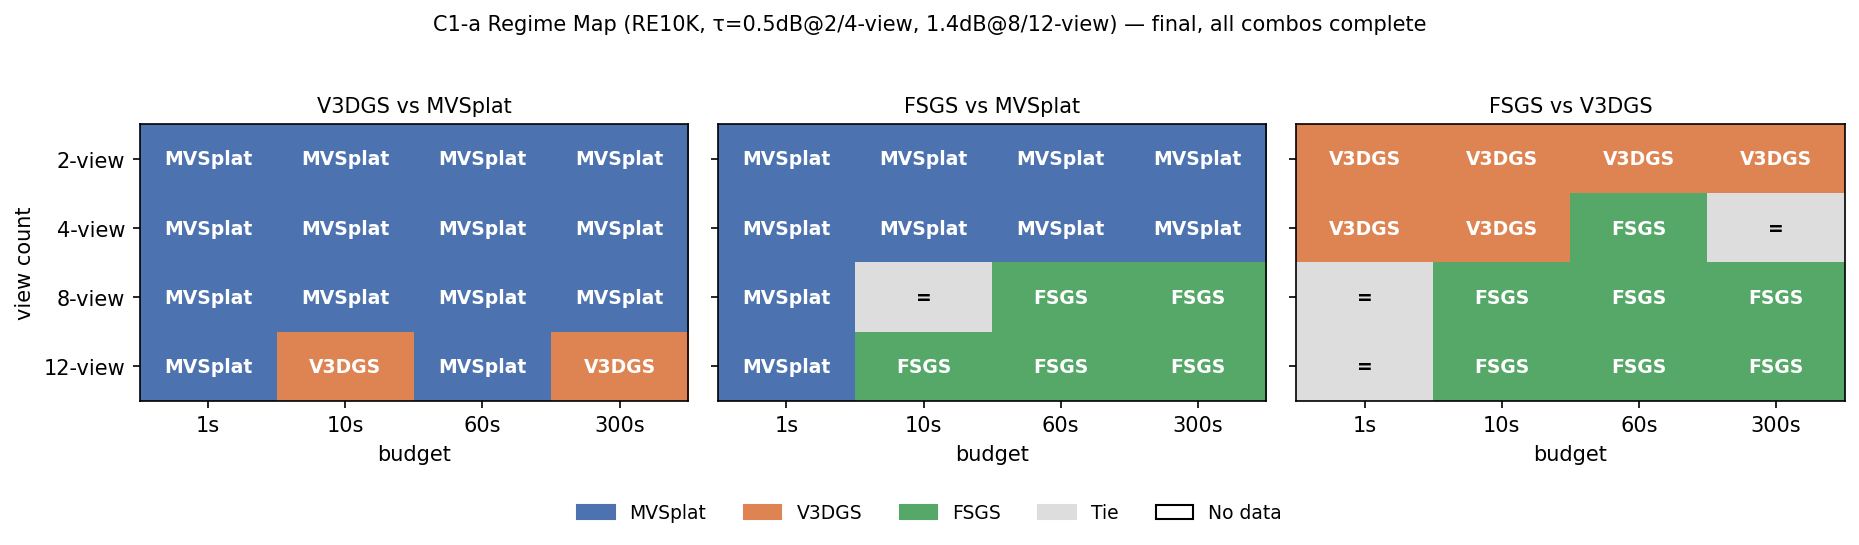
\includegraphics[width=\linewidth]{figures/regime_map.png}
\caption{품질--시간 Regime Map(RE10K 30-scene). 세 방법 쌍(Vanilla3DGS-vs-MVSplat, FSGS-vs-MVSplat, FSGS-vs-Vanilla3DGS) 각각에 대해 $\tau$ 적용 승패 판정(식~\eqref{eq:wtl})을 view 수 $\times$ 예산 격자로 표시. 표~\ref{tab:regime}과 동일한 데이터의 시각화.}
\label{fig:regime-heatmap}
\end{figure}

\subsection{품질--시간 Pareto frontier}

\begin{figure}[h]
\centering
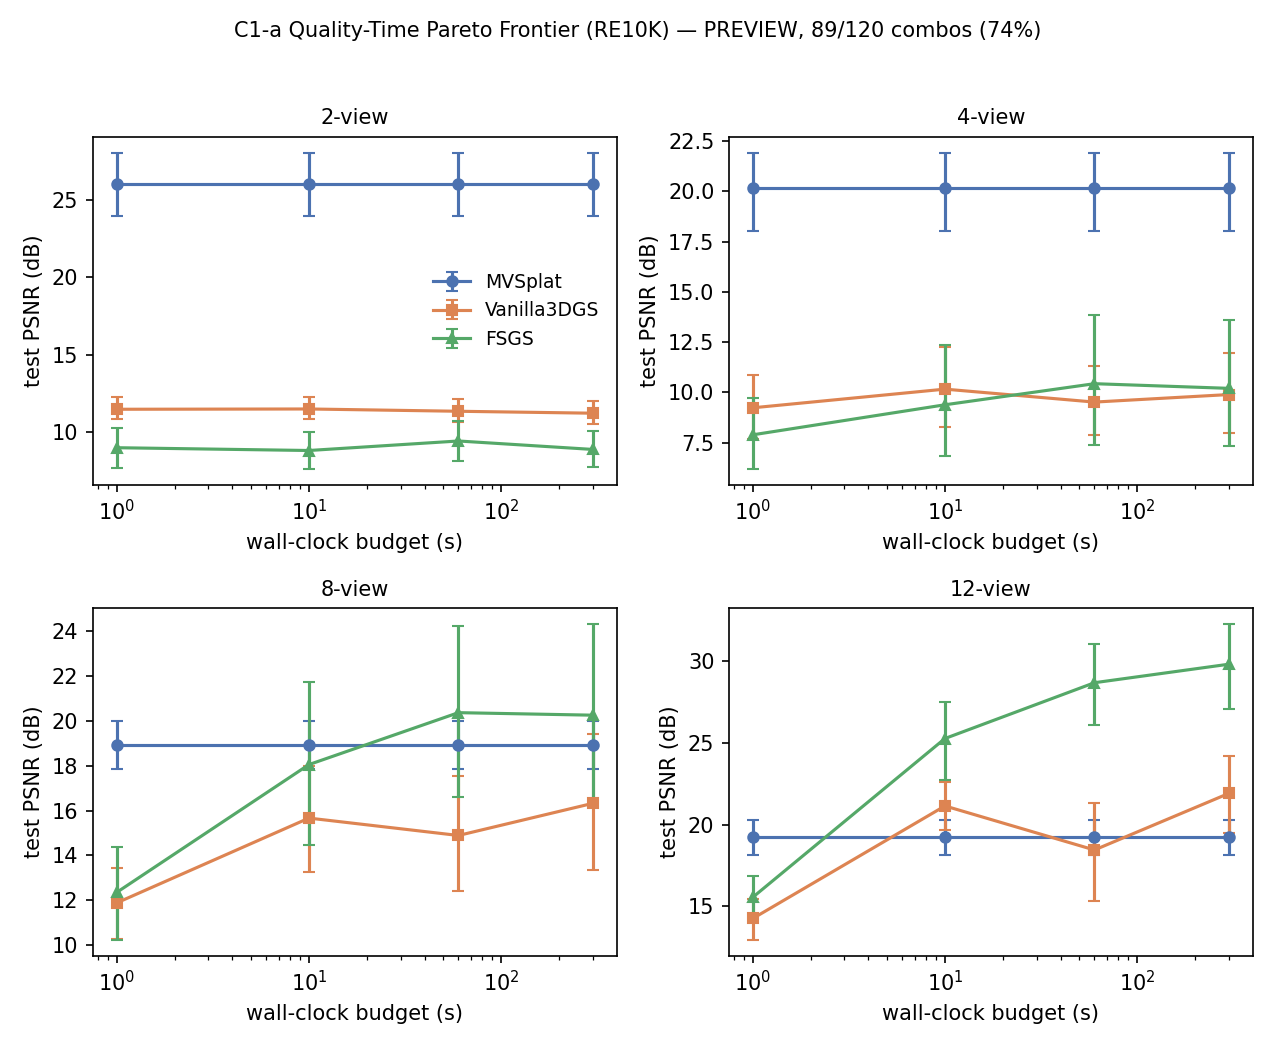
\includegraphics[width=\linewidth]{figures/pareto_frontier.png}
\caption{View 수별(2/4/8/12) 품질--시간 Pareto frontier(RE10K 30-scene). x축 예산(log scale, 1--300s), y축 test PSNR, 오차 막대는 scene cluster bootstrap 95\% CI.}
\label{fig:pareto}
\end{figure}

\subsection{장면별 win rate와 신뢰구간}

표~\ref{tab:regime}의 판정 중 두 지점은 신뢰구간까지 함께 보면 해석이 갈린다.

첫째, FSGS-vs-MVSplat의 8-view 역전은 예산이 늘수록 명확해진다. 60\,s에서 FSGS $20.85$\,dB(95\% CI $[17.48, 24.32]$) 대 MVSplat $18.71$\,dB($[17.79, 19.60]$), 300\,s에서는 FSGS $21.00$\,dB($[17.48, 24.64]$) 대 MVSplat $18.71$\,dB로, 두 CI가 겹치기는 하나 $\Delta$가 $\tau=1.4$\,dB를 넘게 유지되며 scene 수를 30개로 채운 뒤에도 방향이 뒤집히지 않았다(30-scene 이전 부분 데이터에서는 이 경계가 예산에 따라 판정이 흔들렸던 지점이었다).

둘째, 12-view에서 Vanilla3DGS는 예산에 대해 단조롭지 않다 — 10\,s에서 $21.06$\,dB로 MVSplat($19.06$\,dB)을 앞서지만 60\,s에서 $16.97$\,dB로 떨어졌다가 300\,s에 $21.38$\,dB로 회복한다. 이 60\,s 지점의 CI($[14.54, 19.45]$)는 MVSplat의 CI($[18.14, 19.93]$)와 크게 겹쳐 판정 자체는 유지되지만, pooled 평균만으로는 이 비단조성이 개별 scene의 학습 불안정(예: densification/opacity reset 주기와 예산 경계의 우연한 정렬)에서 오는지 체계적 현상인지 구분되지 않는다 — 원인 분석은 \S\ref{sec:failure}에서 다룬다.

\subsection{정성적 비교}

\begin{figure}[h]
\centering
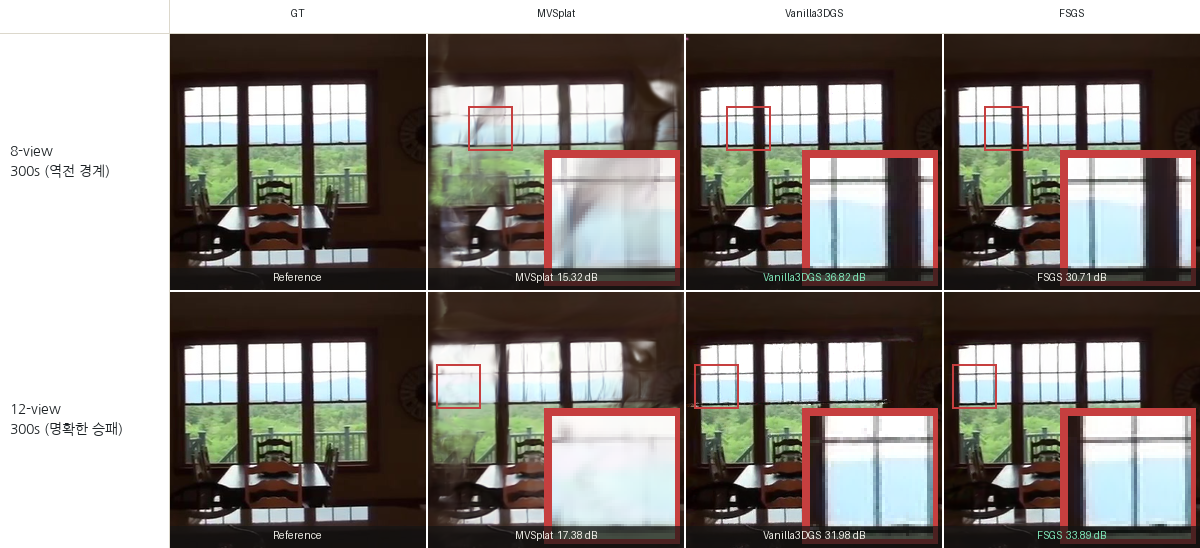
\includegraphics[width=\textwidth]{figures/qualitative_comparison.png}
\caption{RE10K scene \texttt{0588138dfec165a1}에서의 정성적 비교, 왼쪽부터 GT, MVSplat, Vanilla3DGS, FSGS(budget=300\,s). 위 행은 8-view(FSGS-vs-MVSplat 역전 경계 근방, \S\ref{sec:results}), 아래 행은 12-view(FSGS가 명확히 앞서는 조건). 각 패널 하단은 해당 target view의 PSNR(최고값은 초록색), 빨간 박스는 확대 영역(창틀 디테일)이다. MVSplat은 2-view 전용 학습이라 8/12-view 모두 분포 밖(OOD)이며 창틀이 흐릿하게 뭉개지는 것이 확대 영역에서 뚜렷이 보인다 — Vanilla3DGS/FSGS는 두 조건 모두 창틀 선이 살아있고 GT에 훨씬 가깝다.}
\label{fig:qualitative}
\end{figure}

\subsection{동일 초기값 Refinement On/Off}
\label{sec:c1b}

\todo{Feed-forward 출력을 고정한 뒤 refinement off(0\,s)/on(10/60/300\,s) 비교. 렌더 등가성 gate(\S\ref{sec:equivalence}) 통과 조건에서만 진행. 30-scene 최종 설정으로 재실행 필요.}

\subsection{확장 비교: Recurrent Refinement (ReSplat)}
\label{sec:resplat-exploratory}

이 비교군은 사전 등록 설계에 포함되지 않았으며 탐색적 결과로 서술한다. ReSplat~\cite{xu2026resplat}은 DepthSplat과 같은 계보(동일 1저자, 초기화 모델로 DepthSplat 아키텍처를 재사용)이면서 rendering error를 피드백 신호로 삼아 Gaussian을 반복 갱신하는 recurrent refinement 계열이라, 본 연구의 주 비교 두 축(단일 pass feed-forward, per-scene optimization) 어느 쪽에도 온전히 속하지 않는다. 그럼에도 DL3DV에서 저비용으로 실행 가능해(결정론적 단일 추론, scene당 약 1.2\,s) 참고 지점으로 추가했다.

DL3DV 25-scene, C1-a와 동일한 view selection(v2)을 그대로 재사용하고, ReSplat의 8-view 학습 체크포인트(256$\times$448)를 기본으로, 12-view는 16-view 학습 체크포인트도 함께 실행해 분포 이탈 정도를 비교했다.

\begin{table}[h]
\centering
\caption{ReSplat 대 기존 4개 방법, DL3DV 25-scene, budget=300\,s(per-scene 방법 기준). ReSplat 열의 굵은 글씨는 해당 view\_count에서 4개 방법 중 최고값.}
\label{tab:resplat-exploratory}
\begin{tabular}{lcccc}
\toprule
view\_count & ReSplat & DepthSplat & FSGS & Vanilla3DGS \\
\midrule
2  & 14.54\,dB (OOD, 8v ckpt) & \textbf{18.53}\,dB & 11.36\,dB & 11.75\,dB \\
4  & 21.87\,dB (OOD, 8v ckpt) & \textbf{24.01}\,dB & 13.03\,dB & 12.58\,dB \\
8  & \textbf{26.41}\,dB (in-domain) & 25.79\,dB & 24.97\,dB & 19.32\,dB \\
12 & 27.88\,dB (16v ckpt) / 27.42\,dB (8v ckpt) & 25.58\,dB & \textbf{30.07}\,dB & 22.90\,dB \\
\bottomrule
\end{tabular}
\end{table}

8-view(ReSplat의 진짜 in-domain 지점)에서 ReSplat이 4개 방법 중 최고 품질을 낸다 — 같은 아키텍처 계보의 단일 pass DepthSplat보다 +0.6\,dB 높아, recurrent refinement 자체의 이득을 직접 보여준다.

그러나 12-view에서는 16-view 체크포인트를 써도 FSGS(per-scene optimization)가 여전히 2.2\,dB 앞선다 — \S\ref{sec:results}의 핵심 서사(고-view regime에서 per-scene optimization이 feed-forward를 역전)가 더 강한 feed-forward 기준선(ReSplat)을 세워도 유지된다는 뜻이다. 즉 ReSplat은 "feed-forward 계열 중 가장 강하다"이지 "feed-forward가 optimization을 이긴다"는 아니다. 이 8-view 지점은 진짜 in-domain 조건에서 얻은 결과라, \S\ref{sec:ood-confound}에서 논의하는 분포 이탈 confound를 부분적으로 통제한 참고 자료이기도 하다.

Gaussian 수는 view당 DepthSplat의 약 1/16(8-view: 57{,}344 대 917{,}504) 수준으로, ReSplat README가 밝힌 설계(subsampled space 예측)가 실측으로도 확인된다. 다만 peak VRAM은 Gaussian 수만큼 줄지 않는다(recurrent 반복 forward pass 비용).

\begin{figure}[h]
\centering
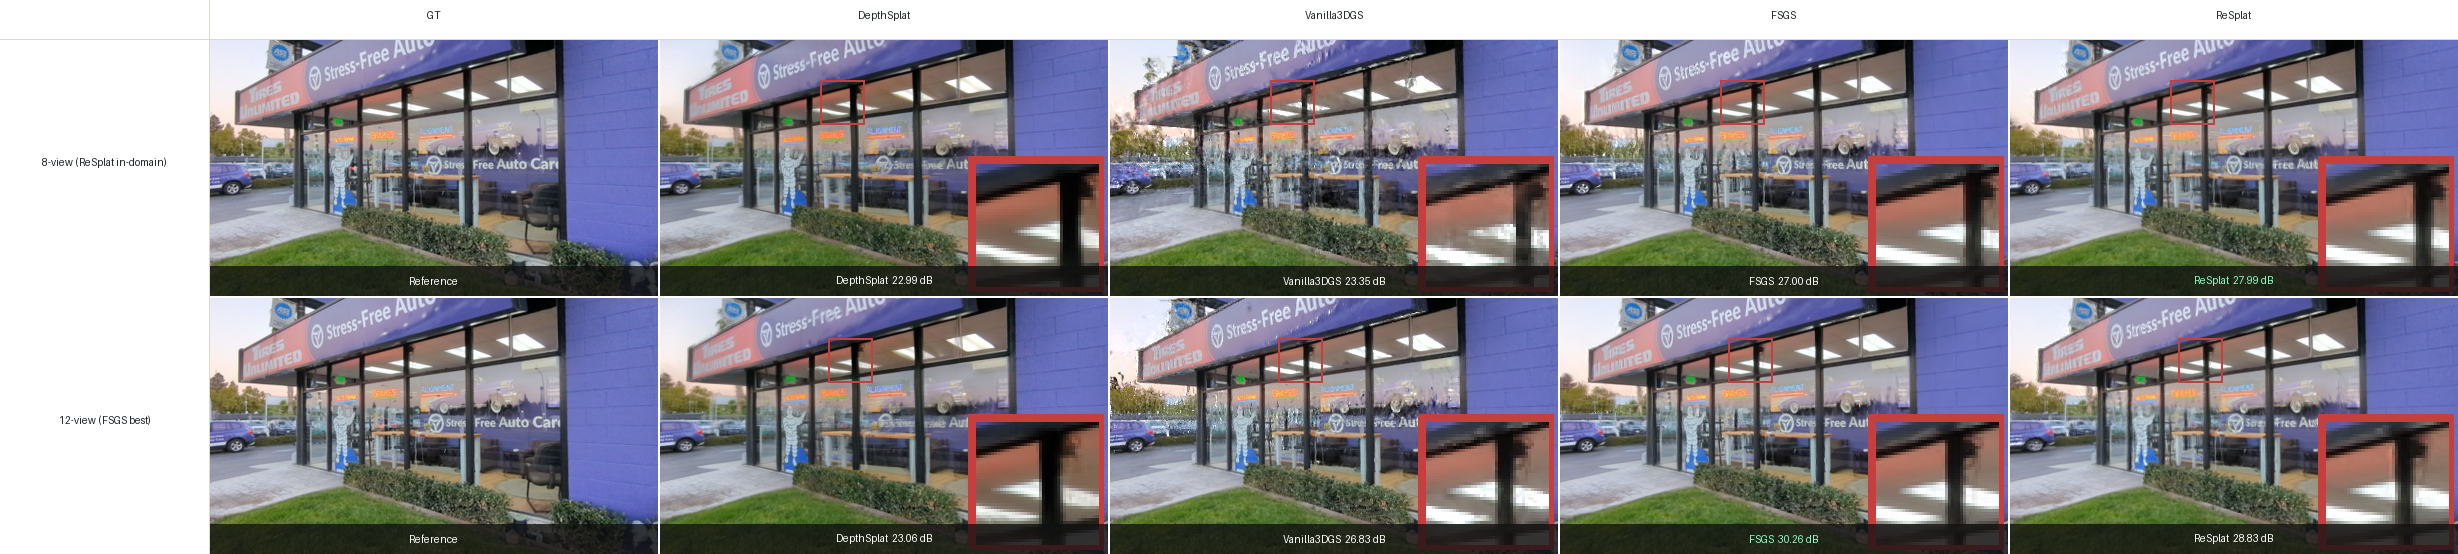
\includegraphics[width=\textwidth]{figures/qualitative_comparison_dl3dv_resplat.png}
\caption{DL3DV scene(§4.2 in-domain 체크포인트 매칭 원칙에 따라 DepthSplat/ReSplat 모두 이 데이터셋으로 학습된 체크포인트 사용)에서 GT/DepthSplat/Vanilla3DGS/FSGS/ReSplat 5개 방법 정성적 비교, budget=300\,s. 위 행은 8-view(ReSplat의 진짜 in-domain 지점, ReSplat이 27.99\,dB로 4개 방법 중 최고), 아래 행은 12-view(FSGS가 30.26\,dB로 최고). 확대 영역(빨간 박스)에서 DepthSplat의 구조물 경계 흐림이 가장 두드러지며, ReSplat은 같은 계보의 DepthSplat보다 뚜렷이 선명하지만 8-view에서도 FSGS와 근소한 차이, 12-view에서는 FSGS에 못 미친다 — 표~\ref{tab:resplat-exploratory}의 수치와 일관된다.}
\label{fig:qualitative-dl3dv-resplat}
\end{figure}

% =====================================================================
\section{실패 분석}
\label{sec:failure}
% =====================================================================

본 절은 Regime Map에서 관찰되는 우위 역전이 \emph{왜} 일어나는지에 대한 메커니즘 수준의 증거를 제시한다.

\subsection{Baseline--overlap--기하 불확실도의 관계}
\label{sec:confound}

두 view로 3D 점을 삼각측량하는 문제는 재투영 오차를 최소화하는 비선형 최소제곱이며, Gauss--Newton 근사 아래에서 추정치의 공분산은 다음과 같이 주어진다~\cite{hartley2003multiple}.
\begin{equation}
\mathrm{Cov}(\hat\beta) \;\approx\; \sigma^2 \bigl(J^\top J\bigr)^{-1}
\label{eq:covariance}
\end{equation}
여기서 $J = \partial r / \partial \beta$는 재투영 오차의 야코비안이고 $\sigma$는 관측 노이즈의 표준편차다. 정렬된 두 view의 단순한 경우 식~\eqref{eq:covariance}의 깊이 성분은 $\sigma_Z \propto Z^2/(fB)$로 정리되며($f$는 초점거리, $B$는 baseline, $Z$는 깊이), 가로 방향 불확실도와의 비는 $\sigma_Z/\sigma_X \propto Z/B$가 된다.

즉 지배 변수는 baseline 자체가 아니라 \textbf{시차비 $B/Z$}이다. 이는 baseline과 overlap이 서로 다른 개념임을 함의한다. Baseline을 키우면 삼각측량 정밀도는 개선되지만 시점 차이가 커져 대응점 탐색이 어려워지고 co-visibility는 감소하므로, 두 요인은 반대 방향으로 작용한다.

이 관계를 실제 데이터에서 진단적으로 검증하였다. DTU scan1의 42-view 재구성에서 모든 view pair(861쌍)에 대해 baseline(카메라 중심 간 거리), overlap(식~\eqref{eq:overlap}), 식~\eqref{eq:covariance} 기반 깊이 불확실도를 계산한 결과, 원시 상관은 $\mathrm{corr}(O_{ij},\ \log\hat\sigma_{\mathrm{depth}}) = +0.952$로 ``overlap이 높을수록 불확실도가 낮다''는 예상과 반대 부호를 보였다.

Baseline을 \emph{선형으로} 통제한 편상관은 $+0.801$로 소폭만 감소했으나, baseline과 불확실도의 관계가 선형이 아니라 거듭제곱 형태임을 확인한 뒤($\mathrm{corr}(\log B,\ \log\hat\sigma) = -0.989$, 선형 버전 $-0.951$) $\log B$로 통제하자 편상관이 $+0.301$로 크게 감소했다.

이 결과의 해석은 두 가지다. 첫째, 부호 역전 자체는 위의 이론과 정합적이다. DTU와 같은 궤도형(orbital) 촬영에서는 두 카메라가 가까울수록 overlap이 크고 동시에 baseline이 작으므로, overlap과 깊이 불확실도가 함께 증가하는 것이 기하학적으로 예측되는 결과다. 둘째, $\log B$ 통제 후에도 잔여 상관 $+0.301$이 남는다는 점은 overlap이 baseline으로 완전히 환원되지는 않음을 시사한다. 따라서 본 연구는 overlap을 주 축으로 유지하되, ``왜 저겹침 조건이 어려운가''에 대한 \emph{설명}은 overlap 자체가 아니라 그 배후의 baseline/parallax 기하에 귀속시킨다.

\begin{figure*}[t]
\centering
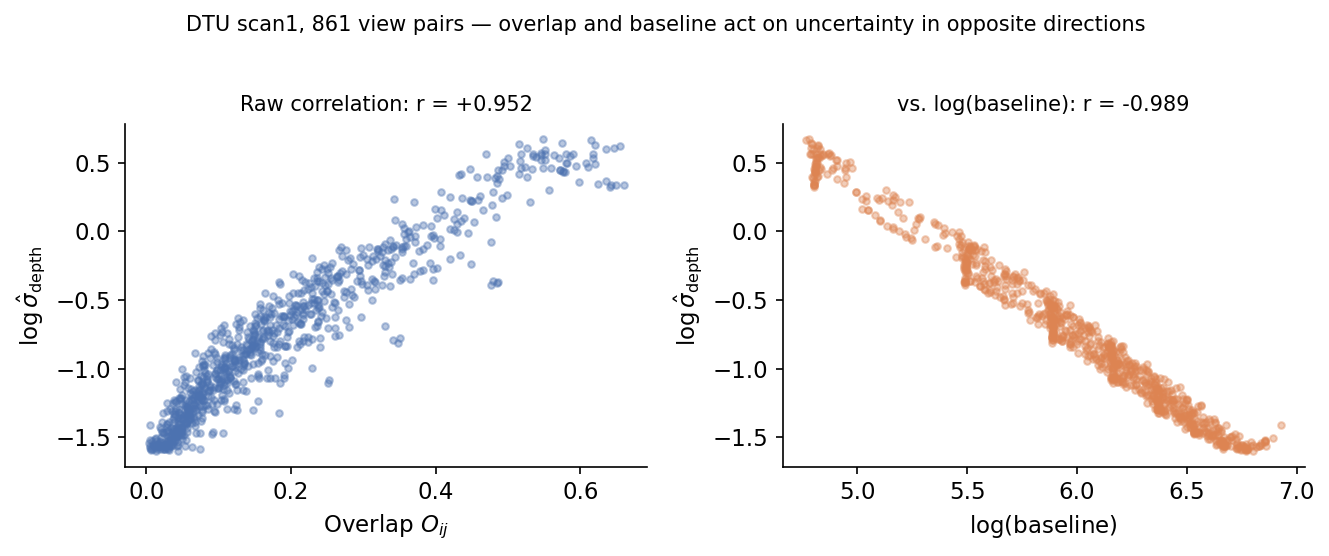
\includegraphics[width=0.8\linewidth]{figures/geometry_confound.png}
\caption{Overlap과 $\log(\mathrm{baseline})$이 깊이 불확실도($\log\hat\sigma_{\mathrm{depth}}$)와 맺는 관계. 왼쪽: 원시 overlap--불확실도 상관은 예상과 반대 부호($r=+0.952$). 오른쪽: $\log(\mathrm{baseline})$과의 관계는 거의 완벽한 선형($r=-0.989$) — baseline 교란이 부호 역전의 주 원인임을 시사한다. DTU scan1, 861 view pair.}
\label{fig:confound}
\end{figure*}

\chk{DTU는 궤도형 rig이므로 overlap과 baseline이 강하게 결합되어 있다. RE10K/DL3DV처럼 경로형(trajectory) 촬영에서는 두 변수의 결합 강도가 다를 수 있으므로 동일 분석을 반드시 반복할 것}

\subsection{Densification gradient의 관측 부족}
\label{sec:starvation}

gsplat~\cite{ye2024gsplat}의 기본 densification 전략은 매 100-iteration window마다 각 Gaussian의 2D 위치 gradient norm 평균을 고정 임계값 $\tau_{\mathrm{pos}} = 2\times 10^{-4}$와 비교해 성장 여부를 결정한다. 이 판단은 $\mathrm{grad2d}[g]\,/\,\mathrm{count}[g]$로 계산되며, $\mathrm{count}[g]$는 해당 Gaussian이 그 window 동안 관측된 횟수(effective observation count)다.

원래 가설은 ``관측이 적은 Gaussian일수록 평균 추정이 노이즈에 취약해 densification을 잘못 유발한다''는 것이었으나, 실측 결과 $\mathrm{count}[g] \le 2$인 Gaussian이 임계값을 초과하는 비율은 모든 조건에서 사실상 0\%(0.00--0.003\%)로 이 가설은 기각되었다. 관측이 적으면 분자인 누적 gradient도 함께 작아지기 때문이다.

대신 \textbf{관측 부족 Gaussian의 비율 자체가 view 수에 강하게 좌우된다}는 것을 발견했다(그림~\ref{fig:starvation}, 표~\ref{tab:starvation}). RE10K 3-scene, 2000-iteration 계측에서 $\mathrm{count}[g] \le 2$인 Gaussian의 비율은 2-view에서 51.5\%, 4-view에서 30.8\%, 8-view에서 3.2\%, 12-view에서 0.7\%로 단조 감소했다. 초기화 방식(COLMAP triangulation 성공 여부에 따른 sparse init 대 random-sphere fallback)이라는 교란요인을 제거하기 위해 4개 view 수 조건 모두 동일하게 random-sphere fallback을 사용한 단일 scene을 별도로 확인한 결과에서도 55.3\% $\to$ 32.3\% $\to$ 8.3\% $\to$ 1.3\%로 같은 패턴이 재현되어, 이 효과가 초기화 방식이 아니라 view 수 자체에 기인함을 확인했다.

\begin{figure}[t]
\centering
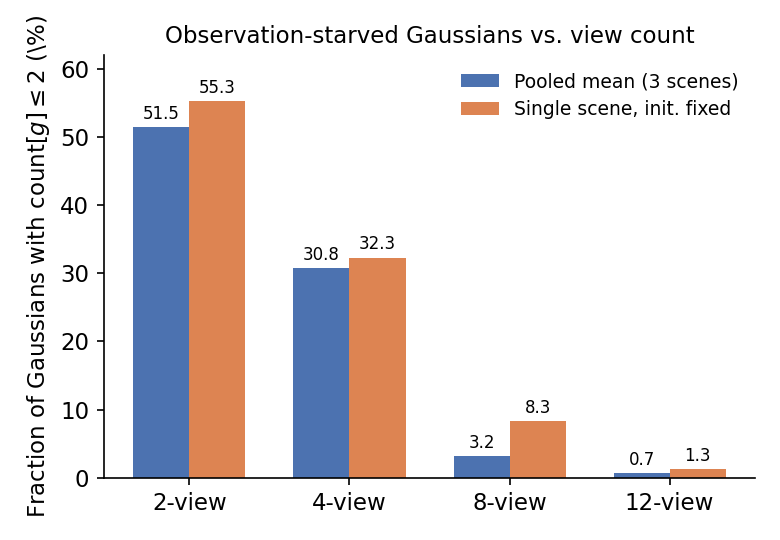
\includegraphics[width=0.95\linewidth]{figures/observation_starvation.png}
\caption{$\mathrm{count}[g] \le 2$인(=최근 100-iteration window에서 2번 이하로만 관측된) Gaussian의 비율. View 수가 늘수록 급격히 감소하며, 초기화 방식(sparse COLMAP init 대 random-sphere fallback)을 고정한 단일 scene에서도 동일한 패턴이 재현된다.}
\label{fig:starvation}
\end{figure}

\begin{table}[h]
\centering
\caption{관측 부족 Gaussian($\mathrm{count}[g] \le 2$)의 비율. RE10K 3-scene, 2000 iteration, seed 0}
\label{tab:starvation}
\small
\begin{tabular}{@{}l cccc@{}}
\toprule
조건 & 2-view & 4-view & 8-view & 12-view \\
\midrule
Pooled 평균 & 51.5\% & 30.8\% & 3.2\% & 0.7\% \\
초기화 고정(단일) & 55.3\% & 32.3\% & 8.3\% & 1.3\% \\
\bottomrule
\end{tabular}
\end{table}

이는 sparse-view에서 optimization이 불리한 이유를 ``데이터가 적다''는 추상적 설명을 넘어, \textbf{Gaussian 예산의 상당 부분이 어떤 학습 구간에서도 유의미한 gradient 신호를 받지 못한 채 방치된다}는 구현 수준에서 추적 가능한 메커니즘으로 제시한다. 이 Gaussian들은 gradient 신호가 미약하여 gradient 기반 densification의 대상이 되지도 못하고, 그렇다고 임계값을 넘어 잘못된 성장을 유발하지도 않으며, 사실상 사용되지 않는 모델 용량으로 남는다.

\chk{현재 결과는 두 원인이 섞여 있을 수 있다. (i) 관측 부족: Gaussian은 적절히 배치되었으나 카메라 수가 적어 소수 view에서만 보이는 경우, (ii) 배치 실패: random-sphere fallback으로 뿌린 점이 애초에 어떤 카메라 절두체에도 포함되지 않는 경우. 어떤 view에도 투영되지 않는 Gaussian의 비율을 별도로 측정해 (ii)를 분리해야 하며, 그 결과에 따라 본 절의 주장이 ``sparse-view 일반의 메커니즘''인지 ``triangulation 실패 시 random 초기화의 한계''인지가 갈린다}

\paragraph{사후 발견으로서의 위치} 본 절의 관측은 사전 등록한 가설 H1--H3에 포함되지 않았던 탐색적 발견(exploratory finding)이다. 따라서 확증적 결과와 구분하여 서술하며, 주 데이터셋 전체 규모에서의 재현 여부를 별도로 보고한다.

\subsection{사전 등록 가설의 검증}
\label{sec:h2-verification}

\begin{table*}[t]
\centering
\caption{사전 등록 가설과 검증 상태}
\label{tab:hypotheses}
\small
\begin{tabular}{@{}l L{12cm} L{2.6cm}@{}}
\toprule
가설 & 내용 & 상태 \\
\midrule
H1 & 초기 geometry 오차($\sigma$)가 커질수록 densification 이후 Gaussian 수는 증가하지만 held-out 품질은 감소하며, 이 관계는 저겹침 조건에서 강화된다 & 절반 지지, 절반 기각(\S\ref{sec:c2}) \\
H2 & Optimization의 품질 정점 도달 시점은 view 수가 줄수록 앞당겨지고, 정점 이후 하강 기울기가 가팔라진다 & 부분 지지 (아래) \\
H3 & 초기 geometry 품질이 일정 수준을 넘으면 refinement의 한계 이득이 소멸한다 & 잠정 지지, 교란 미분리 (\S\ref{sec:c1b}) \\
\bottomrule
\end{tabular}
\end{table*}

세 가설 중 어느 것이 기각되더라도 그 자체가 보고 대상이다. 실제로 \S\ref{sec:starvation}에서 원래 가설(관측 부족으로 인한 오탐)이 기각되고 다른 메커니즘(관측 부족 자체의 비율)이 발견된 사례가 있었다.

\paragraph{H2 검증} RE10K C1-a 궤적 로그(scene당 예산 스냅샷 4개: 1/10/60/300\,s)에서, 4개 지점 중 test PSNR 최댓값이 300\,s 이전(=``조기 정점'')에 나타나는 비율을 view 수별로 집계했다.

\textbf{정점 시점 부분은 지지된다}: 조기 정점 비율은 Vanilla3DGS에서 2-view 91.7\% $\to$ 12-view 63.3\%, FSGS에서 2-view 91.7\% $\to$ 12-view 18.3\%로 두 방법 모두 view 수가 늘수록 단조 감소했다 — view가 적을수록 정점이 일찍 온다는 예측과 일치한다.

그러나 \textbf{하강 기울기 부분은 기각된다}: 조기 정점 발생 시 정점 대비 300\,s 하강폭(scene cluster bootstrap 95\% CI)은 Vanilla3DGS에서 오히려 view 수가 늘수록 커졌다(2-view $0.69\,$dB $[0.45,0.95]$ $\to$ 12-view $2.80\,$dB $[1.88,3.93]$) — 예측과 정반대 방향이다. FSGS에서는 뚜렷한 추세 없이 $0.5$--$0.9\,$dB 범위에 머물렀다(단 12-view는 조기 정점 표본이 scene 7개뿐이라 CI가 넓음).

정점 시점이 앞당겨지는 것과 하강이 가팔라지는 것은 별개 현상이며, 후자는 view 수 자체보다 densification/opacity reset 주기와 예산 경계의 상호작용에 더 좌우되는 것으로 보인다 — 이는 \S\ref{sec:results}에서 관찰한 12-view Vanilla3DGS의 비단조성과 같은 계열의 현상일 가능성이 있다.

\chk{\textbf{표본 해상도의 한계}: 예산 스냅샷이 1/10/60/300\,s 4개뿐이라 ``정점 시점''과 ``하강 기울기'' 추정 모두 해상도가 매우 거칠다 — 실제 정점이 이 4개 지점 \emph{사이}에 있어도 가장 가까운 스냅샷으로만 근사된다. 특히 위 하강폭 결과(view 수가 늘수록 하강이 커짐)는 12-view Vanilla3DGS의 60\,s 지점 비단조성(\S\ref{sec:results}) 자체가 4점 표본에 어떻게 걸리느냐에 따라 만들어졌을 수 있다 — 이 조악한 표본으로는 ``하강이 실제로 view 수에 따라 커진다''와 ``60\,s 근방의 일시적 하락이 우연히 하강폭으로 잡혔다''를 구분할 수 없다. 더 촘촘한 예산 스냅샷(예: 5/15/30/60/120/300\,s)으로 재실행해야 이 둘을 가른다.}

\subsection{Depth 불확실도 개입}
\label{sec:c2}

DTU 8-scan 외부 검증에서 두 종류의 통제된 depth 왜곡을 대표 조건 4개(\texttt{2view\_low\_overlap}, \texttt{4view\_low\_overlap}, \texttt{4view\_high\_overlap}, \texttt{12view\_high\_overlap}) $\times$ seed\{0,1\}에 주입했다: (a) 개별 노이즈 $d' = d(1+\varepsilon)$, $\varepsilon \sim \mathcal{N}(0,\sigma^2)$, $\sigma \in \{0, 0.01, 0.03, 0.05, 0.10\}$, (b) 전역 스케일 편향 $d' = s \cdot d$, $s \in \{0.9, 0.95, 1.0, 1.05, 1.1\}$(단안·저겹침 조건의 절대 스케일 미결정성~\cite{hartley2003multiple}을 모사). 640 combo 전량(2560 rows) 완주했다. 아래는 budget=300\,s 시점, scene cluster bootstrap 기준.

\begin{figure*}[t]
\centering
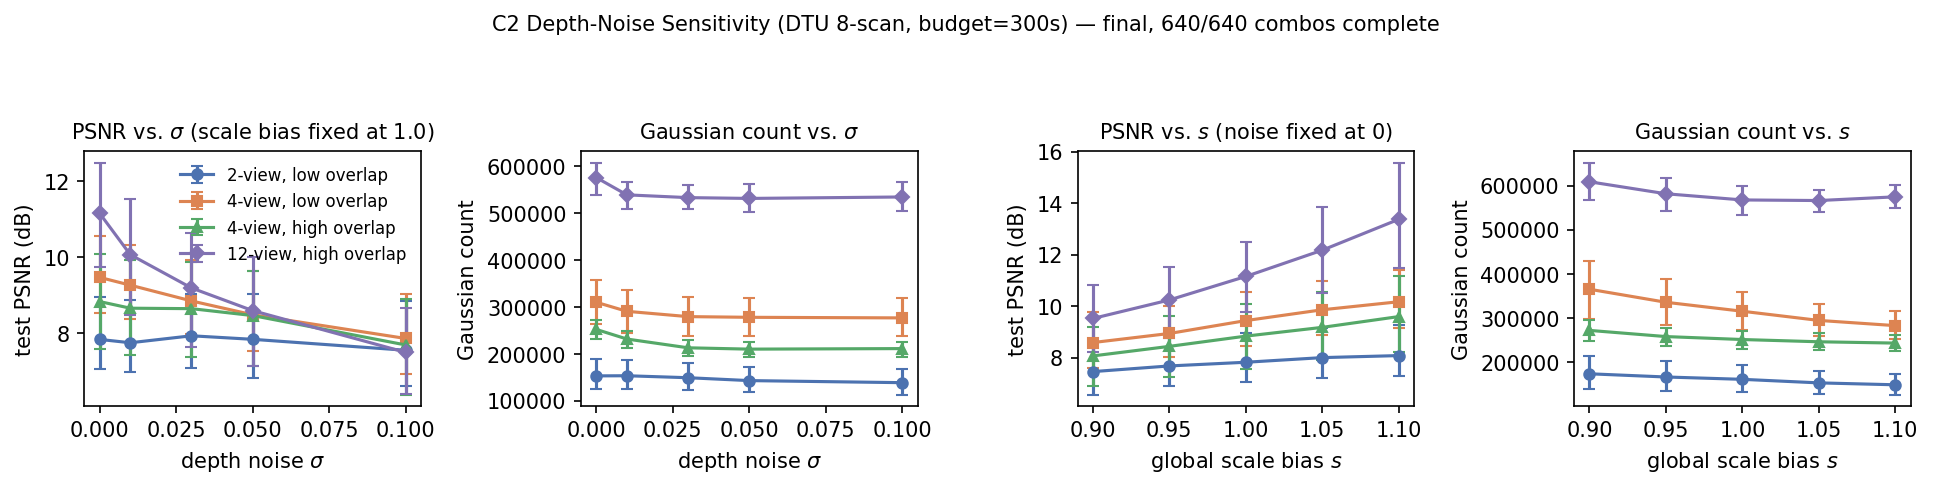
\includegraphics[width=0.85\linewidth]{figures/c2_depth_sensitivity.png}
\caption{C2 depth-noise sensitivity, DTU 8-scan, budget=300\,s. 위 행은 개별 노이즈 $\sigma$ 축, 아래 행은 전역 스케일 편향 $s$ 축. 왼쪽 열(PSNR)은 4개 조건 모두 예측대로 하락(위)/비대칭 단조 증가(아래)하지만, 오른쪽 열(Gaussian 수)은 H1이 예측한 증가가 아니라 하락 또는 평탄이다. 오차 막대는 scene cluster bootstrap 95\% CI.}
\label{fig:c2-sensitivity}
\end{figure*}

\begin{table}[h]
\centering
\caption{H1 예측 대 결과 요약(C2, DTU 8-scan).}
\label{tab:h1-summary}
\small
\begin{tabular}{@{}L{3.3cm} L{3.6cm}@{}}
\toprule
예측 & 결과 \\
\midrule
$\sigma$ $\uparrow$ $\Rightarrow$ PSNR $\downarrow$ & 지지(4개 조건 전부, $r=-0.06$~$-0.51$) \\
$\sigma$ $\uparrow$ $\Rightarrow$ Gaussian 수 $\uparrow$ & 기각 — 반대(4개 조건 전부 하락/평탄, $r=-0.13$~$-0.38$) \\
저겹침에서 두 경향 강화 & 부분 지지($\sigma$축만, 유일 비교쌍인 4-view에서 근소) \\
\bottomrule
\end{tabular}
\end{table}

\paragraph{$\sigma$(개별 노이즈) 축} PSNR은 4개 조건 전부에서 $\sigma$가 커질수록 하락했다(예: 12-view 고겹침 $11.15 \to 7.49\,$dB, $r=-0.51$) — H1의 첫 절반은 지지된다. 그러나 \textbf{Gaussian 수는 4개 조건 전부에서 하락 또는 평탄}했다(예: 12-view 고겹침 $575{,}642 \to 534{,}311$, $r=-0.20$) — ``densification이 나쁜 geometry를 더 많은 Gaussian으로 보정하려 한다''는 두 번째 절반과 정반대다. 노이즈가 gradient 신호 자체를 훼손해 \S\ref{sec:starvation}의 \texttt{count[g]}가 임계값을 덜 넘기게 되고, 그 결과 densification이 오히려 억제되는 것으로 보인다 — \S\ref{sec:starvation}에서 발견한 관측-count 메커니즘과 같은 축의 설명이다.

\paragraph{$s$(전역 스케일 편향) 축} $s=1.0$을 중심으로 대칭적인 U자(0.9와 1.1이 비슷하게 나쁘고 1.0이 최고)를 사전에 기대했으나, 실제로는 \textbf{4개 조건 전부에서 $s=0.9\to1.1$까지 PSNR이 단조 증가}했다(예: 12-view 고겹침 $9.52\to13.37\,$dB) — 탐색 범위 안에서 정점을 찾지 못했다. $s=1.05$/$1.1$이 ``정답 스케일''인 $s=1.0$보다 항상 낫다는 것은, 본 연구의 depth 추정 파이프라인 자체에 계통적 과소추정 편향이 있어 $s>1.0$이 그 편향을 부분 상쇄하고 있을 가능성을 시사한다. 왜곡된 스케일이 ``진짜로 더 좋다''는 결론이 아니라, 탐색 범위를 벗어난 곳에 정점이 있을 가능성을 배제하지 못한다는 뜻으로 해석한다.

\paragraph{Overlap 증폭 효과} 같은 view 수에서 overlap만 다른 직접 비교쌍은 4-view 하나뿐이다(2-view는 저겹침만, 12-view는 고겹침만 설계에 있음). $\sigma$축은 저겹침이 근소하게 더 가파르게 하락했으나($-1.61\,$dB 대 $-1.14\,$dB), $s$축은 사실상 차이가 없었다($+1.59\,$dB 대 $+1.53\,$dB) — H1의 저겹침 증폭 예측은 절반의 절반만 지지된다.

\chk{자세한 조건별 수치와 재현 커맨드는 findings 폴더의 2026-08-19자 C2 분석 문서 참고. $s$축 탐색 범위 확장($s \in \{1.15, 1.2, 1.3\}$)과 Gaussian growth/prune 카운트 분리 계측이 다음 단계로 남아 있다.}

% =====================================================================
\section{실용 가이드라인}
\label{sec:guideline}
% =====================================================================

\todo{\S\ref{sec:results}--\S\ref{sec:failure} 결과가 나온 뒤 채운다. 아래는 형식 예시이며 실제 값은 결과로 대체한다.}

\begin{table}[h]
\centering
\caption{조건별 권장 방법론(형식 예시)}
\label{tab:guideline}
\small
\begin{tabular}{@{}L{7.5cm} l@{}}
\toprule
조건 & 권장 \\
\midrule
view $\le 4$ 이고 overlap이 낮음 & Feed-forward \\
view $\ge 8$ 이고 overlap이 높음 & Per-scene optimization \\
예산 $< 10$초 & Feed-forward \\
예산 $> 300$초이고 초기 geometry 신뢰도가 높음 & Per-scene optimization \\
그 외 & Tie 영역, Pareto frontier 참조 \\
\bottomrule
\end{tabular}
\end{table}

% =====================================================================
\section{결론 및 한계}
\label{sec:conclusion}
% =====================================================================

\todo{전체 결과 요약. 실험 완료 후 작성}

\paragraph{한계}
\begin{itemize}
  \item \textbf{학습 view 분포 이탈}: \S\ref{sec:ood-confound}에서 상술한 대로, view 수를 늘릴 때 feed-forward 모델은 학습 분포를 벗어나는 반면 optimization은 그러한 개념이 없다. 본 연구는 서로 다른 학습 분포를 가진 두 feed-forward 모델의 대조와 동일 초기값 통제 실험으로 이를 완화하지만, 완전히 제거하지는 못한다. 따라서 Regime Map의 결과는 패러다임의 본질적 우열이 아니라 \emph{현재 공개된 대표 체크포인트들의 실용적 우위 영역}으로 해석되어야 한다.
  \item \textbf{Confidence 출력의 비대칭}: 세 방법(MVSplat, DepthSplat, FSGS) 모두 기본 설정에서 실질적인 confidence 출력을 제공하지 않는다. Feed-forward 계열은 관련 출력이 없고, FSGS의 \texttt{confidence} 필드는 기본 설정에서 상수로 고정된 placeholder다. Optimization 쪽은 \S\ref{sec:starvation}의 관측 count를 confidence에 가까운 대체 신호로 사용할 수 있으나, 이는 optimization 계열에만 존재하는 비대칭임을 밝힌다.
  \item \textbf{FSGS 초기화 편차}: 원 논문의 dense-MVS 초기화 대신 sparse COLMAP 초기화를 사용했다. \todo{dense-MVS 초기화를 3--5 scene에 한해 별도 실행해 sparse-init 대비 격차를 정량화하는 보조 검증(낮은 우선순위, COLMAP dense MVS 모듈 확보가 선행 조건)}
  \item \textbf{Overlap 축의 부분 적용}: 본 실험 1단계는 view 수 $\times$ 예산 축으로 수행하고, overlap 축은 selector의 전체 scene 검증 이후 2단계로 추가한다.
  \item \textbf{DL3DV의 pilot 규모}: DL3DV 실험은 공식 10{,}581-scene 전체가 아니라 25-scene pilot subset을 사용한다(공식 평가 split과 중복이 없음은 확인).
  \item \textbf{단일 GPU 예산 제약}: 전체 실험은 약 250 GPU-hour로 추정되며 단일 H200 서버에서 순차 실행된다. 해당 workload가 압도적으로 연산 병목임을 실측으로 확인해(단일 job만으로 GPU 사용률 92--99\%) 다중 프로세스 병렬화로는 총 처리량이 증가하지 않았다.
  \item \textbf{RE10K 데이터 출처}: 확보한 114-scene 중 일부는 원저작자가 아닌 커뮤니티 mirror에서 확보했다. 원 데이터셋과 동일한 chunk 포맷임을 확인하고 공식 체크포인트로 품질을 검증했으나, mirror 자체의 신뢰성은 원저작자가 보증한 것이 아니다.
  \item \textbf{비교 범위}: 본 연구의 주 비교는 단일 pass feed-forward와 per-scene optimization의 두 축이다. ReSplat~\cite{xu2026resplat}처럼 학습된 recurrent 갱신을 사용하는 계열은 별도의 패러다임으로 간주하여 메인 비교에서 제외했다. DL3DV에서 탐색적으로 실행해본 결과(\S\ref{sec:resplat-exploratory}, 사전 등록 설계 밖)는 8-view(in-domain)에서 ReSplat이 DepthSplat을 소폭 능가하지만 12-view에서는 FSGS에 여전히 못 미쳐, 본 연구의 핵심 서사가 더 강한 feed-forward 기준선 아래에서도 유지됨을 시사한다 — 다만 사전 등록되지 않은 단일 실행이라 통제된 비교로 취급하지 않으며, RE10K를 포함한 완전한 통제 비교는 후속 과제로 남긴다.
\end{itemize}

% =====================================================================
\bibliographystyle{plain}
\begin{thebibliography}{99}

\bibitem{kerbl20233d}
Bernhard Kerbl, Georgios Kopanas, Thomas Leimk\"uhler, and George Drettakis.
\newblock 3D Gaussian Splatting for Real-Time Radiance Field Rendering.
\newblock \emph{ACM Transactions on Graphics (Proc. SIGGRAPH)}, 42(4), 2023.

\bibitem{charatan2024pixelsplat}
David Charatan, Sizhe Lester Li, Andrea Tagliasacchi, and Vincent Sitzmann.
\newblock pixelSplat: 3D Gaussian Splats from Image Pairs for Scalable Generalizable 3D Reconstruction.
\newblock In \emph{Proc. IEEE/CVF Conference on Computer Vision and Pattern Recognition (CVPR)}, pages 19457--19467, 2024.

\bibitem{chen2024mvsplat}
Yuedong Chen, Haofei Xu, Chuanxia Zheng, Bohan Zhuang, Marc Pollefeys, Andreas Geiger, Tat-Jen Cham, and Jianfei Cai.
\newblock MVSplat: Efficient 3D Gaussian Splatting from Sparse Multi-View Images.
\newblock In \emph{Proc. European Conference on Computer Vision (ECCV)}, 2024.

\bibitem{xu2025depthsplat}
Haofei Xu, Songyou Peng, Fangjinhua Wang, Hermann Blum, Daniel Barath, Andreas Geiger, and Marc Pollefeys.
\newblock DepthSplat: Connecting Gaussian Splatting and Depth.
\newblock In \emph{Proc. IEEE/CVF Conference on Computer Vision and Pattern Recognition (CVPR)}, 2025.

\bibitem{zhu2024fsgs}
Zehao Zhu, Zhiwen Fan, Yifan Jiang, and Zhangyang Wang.
\newblock FSGS: Real-Time Few-Shot View Synthesis using Gaussian Splatting.
\newblock In \emph{Proc. European Conference on Computer Vision (ECCV)}, 2024.

\bibitem{chen2025splatformer}
Yutong Chen, Marko Mihajlovic, Xiyi Chen, Yiming Wang, Sergey Prokudin, and Siyu Tang.
\newblock SplatFormer: Point Transformer for Robust 3D Gaussian Splatting.
\newblock In \emph{International Conference on Learning Representations (ICLR)}, 2025.

\bibitem{wei2025omniscene}
Dongxu Wei, Zhiqi Li, and Peidong Liu.
\newblock Omni-Scene: Omni-Gaussian Representation for Ego-Centric Sparse-View Scene Reconstruction.
\newblock In \emph{Proc. IEEE/CVF Conference on Computer Vision and Pattern Recognition (CVPR)}, 2025.

\bibitem{liu2026diff3r}
Yueh-Cheng Liu, Jozef Hladk\'{y}, Matthias Nie{\ss}ner, and Angela Dai.
\newblock Diff3R: Feed-forward 3D Gaussian Splatting with Uncertainty-aware Differentiable Optimization.
\newblock \emph{arXiv preprint arXiv:2604.01030}, 2026.
% 2026-08-13 웹서치로 저자/venue 확인 완료(arXiv 프리프린트가 맞음). 이름 오타(Hlad\'{y}->Hladk\'{y}) 수정.

\bibitem{li2026foresplat}
Yuke Li, Weihang Liu, Cheng Zhang, Yuefeng Zhang, Jiadi Cui, Zixuan Wang, Junran Ding, Haoyu Wu, Yujiao Shi, Jingyi Yu, and Xin Lou.
\newblock ForeSplat: Optimization-Aware Foresight for Feed-Forward 3D Gaussian Splatting.
\newblock \emph{arXiv preprint arXiv:2605.22020}, 2026.
% 2026-08-13 웹서치로 전체 11인 저자 목록 확인 완료(arXiv abstract 페이지 직접 대조).

\bibitem{xu2026resplat}
Haofei Xu, Daniel Barath, Andreas Geiger, and Marc Pollefeys.
\newblock ReSplat: Learning Recurrent Gaussian Splatting.
\newblock \emph{Proc. European Conference on Computer Vision (ECCV)}, 2026.
% 2026-08-14 웹서치+arXiv abstract 직접 대조로 저자 4인 확인(arXiv:2510.08575). 1저자가
% DepthSplat 1저자와 동일 인물. abstract 수준에서는 "per-scene optimization이 sparse-view에서
% 실패한다"를 직접 비교하기보다 "feed-forward를 반복적으로 개선"하는 접근으로 스스로를 위치시킴
% — 본문 서술(위 관련연구 절)도 이 구분을 정확히 반영해서 썼음(과장 없이).

\bibitem{yao2018mvsnet}
Yao Yao, Zixin Luo, Shiwei Li, Tian Fang, and Long Quan.
\newblock MVSNet: Depth Inference for Unstructured Multi-view Stereo.
\newblock In \emph{Proc. European Conference on Computer Vision (ECCV)}, 2018.

\bibitem{schoenberger2016sfm}
Johannes L. Sch\"onberger and Jan-Michael Frahm.
\newblock Structure-from-Motion Revisited.
\newblock In \emph{Proc. IEEE Conference on Computer Vision and Pattern Recognition (CVPR)}, 2016.

\bibitem{ye2024gsplat}
Vickie Ye, Ruilong Li, Justin Kerr, Matias Turkulainen, Brent Yi, Zhuoyang Pan, Otto Seiskari, Jianbo Ye, Jeffrey Hu, Matthew Tancik, and Angjoo Kanazawa.
\newblock gsplat: An Open-Source Library for Gaussian Splatting.
\newblock \emph{arXiv preprint arXiv:2409.06765}, 2024.

\bibitem{zhou2018stereo}
Tinghui Zhou, Richard Tucker, John Flynn, Graham Fyffe, and Noah Snavely.
\newblock Stereo Magnification: Learning View Synthesis using Multiplane Images.
\newblock \emph{ACM Transactions on Graphics (Proc. SIGGRAPH)}, 37(4), 2018.

\bibitem{ling2024dl3dv}
Lu Ling, Yichen Sheng, Zhi Tu, Wentian Zhao, Cheng Xin, Kun Wan, Lantao Yu, Qianyu Guo, Zixun Yu, Yawen Lu, et al.
\newblock DL3DV-10K: A Large-Scale Scene Dataset for Deep Learning-based 3D Vision.
\newblock In \emph{Proc. IEEE/CVF Conference on Computer Vision and Pattern Recognition (CVPR)}, pages 22160--22169, 2024.

\bibitem{jensen2014dtu}
Rasmus Jensen, Anders Dahl, George Vogiatzis, Engin Tola, and Henrik Aan{\ae}s.
\newblock Large Scale Multi-view Stereopsis Evaluation.
\newblock In \emph{Proc. IEEE Conference on Computer Vision and Pattern Recognition (CVPR)}, pages 406--413, 2014.

\bibitem{ranftl2022midas}
Ren\'{e} Ranftl, Katrin Lasinger, David Hafner, Konrad Schindler, and Vladlen Koltun.
\newblock Towards Robust Monocular Depth Estimation: Mixing Datasets for Zero-shot Cross-dataset Transfer.
\newblock \emph{IEEE Transactions on Pattern Analysis and Machine Intelligence}, 44(3), 2022.

\bibitem{hartley2003multiple}
Richard Hartley and Andrew Zisserman.
\newblock \emph{Multiple View Geometry in Computer Vision}.
\newblock Cambridge University Press, 2nd edition, 2003.

\bibitem{wang2004ssim}
Zhou Wang, Alan C. Bovik, Hamid R. Sheikh, and Eero P. Simoncelli.
\newblock Image Quality Assessment: From Error Visibility to Structural Similarity.
\newblock \emph{IEEE Transactions on Image Processing}, 13(4):600--612, 2004.

\bibitem{zhang2018lpips}
Richard Zhang, Phillip Isola, Alexei A. Efros, Eli Shechtman, and Oliver Wang.
\newblock The Unreasonable Effectiveness of Deep Features as a Perceptual Metric.
\newblock In \emph{Proc. IEEE Conference on Computer Vision and Pattern Recognition (CVPR)}, pages 586--595, 2018.

\bibitem{holm1979simple}
Sture Holm.
\newblock A Simple Sequentially Rejective Multiple Test Procedure.
\newblock \emph{Scandinavian Journal of Statistics}, 6(2):65--70, 1979.

\bibitem{efron1993bootstrap}
Bradley Efron and Robert J. Tibshirani.
\newblock \emph{An Introduction to the Bootstrap}.
\newblock Chapman \& Hall/CRC, 1993.

\end{thebibliography}


\end{document}
